\documentclass[11pt]{article}

\usepackage[a4paper,margin=1in]{geometry}
\usepackage{amsmath}
\usepackage{amssymb}
\usepackage{array}
\usepackage{booktabs}
\usepackage{float}
\usepackage{graphicx}
\usepackage{xcolor}
\usepackage[colorlinks=true,linkcolor=blue,citecolor=blue,urlcolor=blue]{hyperref}

\newcommand{\Syn}{P_{\mathrm{Syn}}}
\newcommand{\Comp}{P_{\mathrm{Comp}}}
\newcommand{\Words}{P_{\mathrm{WordsSyn}}}
\newcommand{\Rand}{P_{\mathrm{Rand}}}

\title{Have Newer Models Learned to Read Idioms?\\[2pt]
\large A Re-examination of Idiomaticity in Word Representations,
from 2024 Encoders to 2026 LLMs, Calibrated Against Ordinary Perturbations}
\author{First draft for review}
\date{\today}

\begin{document}
\maketitle
\thispagestyle{empty}

\begin{abstract}
An idiom like \emph{grey matter} means ``brain,'' not ``material that is grey.'' He et
al.~(2025) showed that 2024-era word-representation models do not encode such holistic meanings:
when the compound is swapped for its gold synonym, models often find the literal pieces
(\emph{matter}, \emph{silvery material}) closer than the correct paraphrase. We ask whether the
rapid progress since then has changed this. We rebuild their minimal-pair probe as a model-agnostic
framework and run it on twenty models: multilingual encoders, the strongest 2025 and 2026
sentence-embedding models, and a decoder-only LLM cohort (Qwen3, Qwen3.5, Gemma~3, Gemma~4; base and
instruction-tuned; 0.8B to 12B), on English and Portuguese. To run linear-attention and multimodal
LLMs on Apple Silicon we add an MLX path and a layer-recording recipe that we show is essential for
these models. We find a soft ceiling. Every model scores below the partial-capture threshold; the
best, base Gemma~4-12B, reaches only $0.525$ while becoming the first model to actually prefer the
gold synonym over the literal one. We then add the control the original protocol lacks: the same
synonym-versus-random test on ordinary, non-idiomatic words (\emph{doctor} to \emph{physician} vs
\emph{carpet}) and phrases. No model separates idiomatic synonyms from random replacements as well
as it does for ordinary targets. This calibration is the strongest evidence that the failure is
specific to idiomaticity, not a generic insensitivity of embeddings, and that scale and newer
generations approach but do not cross the bar.
\end{abstract}

\section{Introduction}

\paragraph{The problem in one sentence.} A multiword expression is \emph{idiomatic} when its
meaning cannot be recovered from its parts. \emph{Grey matter} is the brain; \emph{red tape} is
bureaucracy; a \emph{cash cow} is a reliable source of money. A model that truly ``understands''
such an expression should place it, in its representation space, near its real meaning (near
\emph{brain}, \emph{bureaucracy}, \emph{reliable earner}) and far from a literal re-reading of its
words. The question of this paper is simple to state: do today's models do this, and have the last
two years of progress helped?

\paragraph{Why this is not obvious to test.} You cannot just ask a model ``is \emph{grey matter}
idiomatic?,'' because that tests its chat behaviour, not its representations. He et
al.~\cite{he2025idiomaticity} instead use a \emph{minimal-pair probe}: take a sentence containing
the compound, replace the compound with carefully chosen substitutes, and measure how much the
representation moves. If replacing \emph{grey matter} with \emph{brain} (its correct meaning)
barely changes the representation, but replacing it with \emph{matter} (a literal piece) changes it
a lot, the model has understood the idiom. Their finding was negative: 2024 models behaved the
opposite way. We revisit that finding with newer and larger models, and we add a control that the
original protocol was missing.

\paragraph{Contributions.} This paper makes four contributions.
\begin{enumerate}
  \item A model-agnostic re-implementation of the NCIMP probe and its metrics, with an MLX backend
  that lets linear-attention (Qwen3.5) and multimodal (Gemma~4) LLMs run on Apple Silicon, and a
  layer-recording recipe we show is necessary to get a fair representation from decoder LLMs
  (Section~\ref{sec:framework}).
  \item Four experiments under one protocol: replicating the paper on 2024 encoders in two
  languages (Section~\ref{sec:exp1}); 2025 and 2026 sentence-embedding models
  (Section~\ref{sec:exp2}); an eleven-model decoder-LLM cohort (Section~\ref{sec:exp3}); and an
  ordinary-perturbation control on all twenty models (Section~\ref{sec:exp4}).
  \item A single, calibrated answer: a soft ceiling around $0.50$ to $0.53$ that nothing crosses,
  with the failure shown to be specific to idiomaticity rather than a generic embedding artefact
  (Section~\ref{sec:discussion}).
  \item Two methodological findings that matter for anyone probing modern LLMs: the final-layer
  residual stream of decoder LLMs must be normalised before it can be measured, and the composite
  capture score must be read together with an anisotropy diagnostic.
\end{enumerate}
Section~\ref{sec:probe} introduces the probe on a single sentence and Section~\ref{sec:metrics} the
metrics; Section~\ref{sec:framework} describes the framework; the four experiments follow; and
Section~\ref{sec:together} collects all twenty models in one table before the discussion.

\section{The Probe, by Example}
\label{sec:probe}

We introduce the method on one concrete sentence before giving any formulas. Take the idiomatic
compound \emph{grey matter} in
\begin{quote}
\emph{``These youngsters use their grey matter when the presentation is right.''}
\end{quote}
The probe replaces the target compound (the \emph{noun compound}, NC) with four kinds of substitute,
each chosen to test a specific expectation.
\begin{itemize}
  \item $\Syn$, the \textbf{gold holistic synonym}: \emph{grey matter} to \emph{brain}. This
  preserves the real meaning, so similarity \emph{should be high} regardless of how idiomatic the
  compound is.
  \item $\Comp$, the \textbf{single most informative component}: \emph{grey matter} to \emph{matter}.
  A part of the compound. For an idiom this loses the meaning, so similarity \emph{should be low};
  for a compositional compound it may stay high.
  \item $\Words$, a \textbf{word-by-word literal synonym}: \emph{grey matter} to \emph{silvery
  material}. Each word replaced by an out-of-context synonym. For an idiom this gives nonsense, so
  similarity \emph{should be low}.
  \item $\Rand$, a \textbf{frequency-matched random expression}: \emph{grey matter} to
  \emph{battlefront serviceman}. Unrelated; a lower-bound control, similarity \emph{should be
  lowest}.
\end{itemize}

So the pattern an idiomaticity-aware model \emph{should} produce is: $\Syn$ high, then ($\Comp$,
$\Words$) middling, then $\Rand$ low. Table~\ref{tab:worked} shows what one real model (BGE-M3)
actually does, next to a compositional compound for contrast.

\begin{table}[H]
\centering
\small
\begin{tabular}{llrl}
\toprule
Compound & Substitution (probe) & $\cos$ & What should happen \\
\midrule
\emph{grey matter} & \emph{brain} \;($\Syn$) & 0.55 & highest, but here it is the lowest non-random \\
(idiomatic) & \emph{matter} \;($\Comp$) & \textbf{0.78} & low, but here it is the highest \\
 & \emph{silvery material} \;($\Words$) & 0.64 & low, but here it beats the gold synonym \\
 & \emph{battlefront serviceman} \;($\Rand$) & 0.47 & lowest, ok \\
\midrule
\emph{economic aid} & \emph{financial assistance} \;($\Syn$) & \textbf{0.81} & highest, ok \\
(compositional) & \emph{aid} \;($\Comp$) & 0.73 & (allowed to be high) \\
 & \emph{budgetary assistance} \;($\Words$) & 0.76 & (allowed to be high) \\
 & (random) \;($\Rand$) & 0.47 & lowest, ok \\
\bottomrule
\end{tabular}
\caption{The whole study in one table (BGE-M3, contextual-span level). For the compositional
\emph{economic aid}, the gold synonym is correctly the closest substitute ($0.81$). For the
idiomatic \emph{grey matter}, the model puts the literal component \emph{matter} ($0.78$) and the
word-by-word \emph{silvery material} ($0.64$) closer than the correct \emph{brain} ($0.55$): it
reads the idiom as the sum of its parts.}
\label{tab:worked}
\end{table}

\paragraph{The dataset (NCIMP).} The compounds come from the Noun Compound Idiomaticity Minimal
Pairs dataset~\cite{he2025idiomaticity}: 280 English and 180 Portuguese compounds, each labelled by
humans on a 0 (fully idiomatic) to 5 (fully compositional) scale and placed in three natural
sentences plus an uninformative ``neutral'' template. Table~\ref{tab:data} lists representative
items in each class. We use the human compositionality score, denoted $\mathrm{Comp}$, as the gold
standard, and we report results at the NC level (the contextual span of the compound), which the
paper finds most diagnostic.

\begin{table}[H]
\centering
\small
\begin{tabular}{lll}
\toprule
Class & Example compound & Example sentence \\
\midrule
Idiomatic & \emph{grey matter} (brain) & ``\dots use their \textbf{grey matter} when the presentation is right.'' \\
Idiomatic & \emph{eager beaver} (hard worker) & ``Eric was being an \textbf{eager beaver} and left work late.'' \\
Partly comp. & \emph{Dutch courage} (courage from drink) & ``\dots go down to the pub to get some \textbf{Dutch courage}.'' \\
Compositional & \emph{economic aid} (financial help) & ``\dots giving Cuba \textbf{economic aid} and military support.'' \\
Compositional & \emph{research lab} (research facility) & ``Being part of a \textbf{research lab} provides fieldwork.'' \\
\bottomrule
\end{tabular}
\caption{Representative NCIMP items. Each compound is probed with the four substitutes of
Section~\ref{sec:probe}.}
\label{tab:data}
\end{table}

\section{Metrics, Each With Its Example}
\label{sec:metrics}

All metrics build on cosine similarity between two representation vectors. We keep using the
\emph{grey matter} numbers from Table~\ref{tab:worked} ($\Syn=0.55$, $\Comp=0.78$, $\Words=0.64$,
$\Rand=0.47$) so every definition is concrete.

\paragraph{Similarity ($S$).} The raw cosine between the original NC representation and the
probe-modified one, $S(P_i) = \cos(e(P_i), e(\mathrm{NC}))$. \emph{Example:} $S(\Syn)=\cos(\text{grey
matter},\text{brain})=0.55$.

\paragraph{Affinity ($A$).} Which of two probes is closer? $A(P_i,P_j)=S(P_i)-S(P_j)$. \emph{Example:}
$A(\Syn,\Words)=0.55-0.64=-0.09$. The negative sign says the model prefers the literal ``silvery
material'' to the correct ``brain,'' exactly the wrong preference.

\paragraph{Scaled similarity ($S^R$).} Embedding spaces are anisotropic, so even random vectors can
look similar and a raw $0.55$ is hard to read. We rescale against the random floor,
\[
S^R(P_i) = \frac{S(P_i)-S(\Rand)}{\,1-S(\Rand)\,}.
\]
\emph{Example:} $S^R(\Syn)=(0.55-0.47)/(1-0.47)=0.15$. So the gold synonym sits only $15\%$ of the
way from ``random'' to ``identical,'' meaning the holistic meaning is almost not recovered.

\paragraph{Per-model diagnostics.} Averaging over the idiomatic compounds gives four readable
numbers, each with a clear ideal direction (Table~\ref{tab:metricdef}).

\begin{table}[H]
\centering
\small
\begin{tabular}{lll}
\toprule
Metric & Meaning & Ideal \\
\midrule
ISC & idiomatic synonym capture, $\overline{S^R(\Syn)}$ on idioms & high (near 1) \\
LOD & lexical-overlap dominance, $\overline{S^R(\Words)-S^R(\Syn)}$ & below 0 \\
FLOOR & random-similarity floor, $\overline{S(\Rand)}$ (anisotropy) & diagnostic \\
ISC$\to$ICS & composite capture score in $[0,1]$ & high; $\ge0.55$ partial, $\ge0.70$ captures \\
\bottomrule
\end{tabular}
\caption{The four diagnostics, illustrated on \emph{grey matter}: ISC asks ``is \emph{brain}
recovered?''; LOD is positive here ($\Words\,0.64 > \Syn\,0.55$), the component-bias failure; FLOOR
asks ``does \emph{battlefront serviceman} also look similar?''; ICS rolls these into one score.}
\label{tab:metricdef}
\end{table}

\paragraph{A caveat we will need (anisotropy breaks the composite).} Because $S^R$ divides by
$1-\mathrm{FLOOR}$, the composite becomes unstable as $\mathrm{FLOOR}$ approaches $1$. \emph{Example:}
a model whose space has collapsed to $\mathrm{FLOOR}=0.95$ has a denominator of $0.05$, so tiny
noise is amplified and the indicators drift to ``neutral,'' which the composite can mistake for a
decent score. We meet exactly this case (instruction-tuned Gemma~4-12B in Section~\ref{sec:exp3})
and therefore always report FLOOR next to ICS.

\section{The Model-Agnostic Framework}
\label{sec:framework}

The probe and the metrics are held fixed; only the model changes. Each model is wrapped as an
\emph{embedder} exposing two operations: embed a whole sentence, and embed the target span within
its sentence (mean-pooling the relevant sub-tokens over the last four layers, following the original
protocol). Table~\ref{tab:embedders} lists the embedder types; static vectors, transformer encoders,
sentence-embedding models, and decoder-only LLMs all fit one interface, so the probe code never
changes between a 2024 encoder and a 2026 LLM.

\begin{table}[H]
\centering
\small
\begin{tabular}{lll}
\toprule
Embedder type & Runtime & Used for \\
\midrule
transformer & HuggingFace/torch & BERT, mBERT, DistilBERT, XLM-R \\
sentence & sentence-transformers & mSBERT, BGE-M3, E5, Qwen3-Embedding \\
causal & HuggingFace/torch & Qwen3, Gemma~4-E2B (text path) \\
mlx\_causal & Apple MLX (mlx-lm / mlx-vlm) & Qwen3.5, Gemma~3, Gemma~4-12B \\
\bottomrule
\end{tabular}
\caption{Pluggable embedder types. Adding a model is one registry line; the probe and metrics are
untouched, which is what makes the cross-generation comparison fair.}
\label{tab:embedders}
\end{table}

\paragraph{Why an MLX path was needed.} Two of the newest LLM families do not run well through the
standard PyTorch path on Apple Silicon. Qwen3.5 uses linear attention whose fast kernels are
CUDA-only, so PyTorch falls back to an unusably slow implementation; and Gemma~4 is a unified
multimodal architecture (\texttt{gemma4\_unified}) that the text-only loader rejects. We therefore
added an MLX embedder that loads text LLMs via \texttt{mlx-lm} and multimodal ones via
\texttt{mlx-vlm}, converting the base checkpoints on the fly so we keep full-precision base weights.
On an M2~Max this turns a multi-hour or impossible run into minutes.

\paragraph{Why the last layer alone is not enough, and the fix.} MLX exposes only the final hidden
state cheaply, but for decoder LLMs the final-layer residual stream is pathologically anisotropic.
\emph{Example:} for base Gemma~3-12B, the cosine between two unrelated sentences, \emph{``grey matter
functioning here''} and \emph{``supermarket city raining now,''} is $0.98$ from the raw last-four
layers; everything looks alike. The cause is a large shared component that the model's own final
RMSNorm is designed to remove. Recording the last four decoder layers and then applying that final
norm drops the same cosine to $0.56$ and restores a usable representation. We use this
last-four-layers-plus-final-norm recipe for all MLX models; it is the difference between a meaningful
score and noise, and it is one of the two methodological findings of this paper.

\section{Experiment 1: Replicating the Paper on 2024 Encoders}
\label{sec:exp1}

\paragraph{Setup.} Six multilingual models in two cohorts: paper-era (mBERT, multilingual
DistilBERT, mSBERT) and 2024-modern (XLM-R-large, BGE-M3, multilingual~E5-large), on English (1124
instances) and Portuguese (720), at NC level.

\paragraph{Expected vs.\ actual.} As in Section~\ref{sec:probe}, the gold synonym should be the
closest substitute for every class, while the literal probes should fall off for idioms.
Table~\ref{tab:worked} already showed the failure on \emph{grey matter} and the success on
\emph{economic aid} for one of these models. Aggregated by cohort (Table~\ref{tab:enccohort}) and by
model (Table~\ref{tab:encmodel}), the picture is uniform: English improves modestly from the older
to the newer cohort, Portuguese does not, and no model crosses $0.55$.

\begin{table}[H]
\centering
\small
\begin{tabular}{llrrr}
\toprule
Lang. & Cohort & ISC & LOD & ICS \\
\midrule
EN & paper-era (mBERT, DistilBERT-ML, mSBERT) & 0.099 & 0.227 & 0.341 \\
EN & 2024-modern (XLM-R, BGE-M3, E5-large) & 0.174 & 0.077 & 0.430 \\
PT & paper-era & 0.150 & 0.203 & 0.428 \\
PT & 2024-modern & 0.095 & 0.158 & 0.423 \\
\bottomrule
\end{tabular}
\caption{Encoder cohorts at NC level (mean over naturalistic and neutral contexts). English gains
modestly ($0.341$ to $0.430$); Portuguese is flat. LOD stays positive throughout: the literal pieces
beat the holistic synonym for idioms in every cohort.}
\label{tab:enccohort}
\end{table}

\begin{table}[H]
\centering
\small
\begin{tabular}{lrrrr|rrrr}
\toprule
 & \multicolumn{4}{c|}{English} & \multicolumn{4}{c}{Portuguese} \\
Model & ISC & LOD & FLOOR & ICS & ISC & LOD & FLOOR & ICS \\
\midrule
mBERT          & 0.085 & 0.205 & 0.777 & 0.353 & 0.125 & 0.191 & 0.795 & 0.435 \\
DistilBERT-ML  & 0.021 & 0.181 & 0.744 & 0.349 & 0.004 & 0.191 & 0.779 & 0.419 \\
mSBERT         & 0.191 & 0.295 & 0.205 & 0.320 & 0.322 & 0.228 & 0.250 & 0.431 \\
XLM-R-large    & 0.100 & 0.071 & 0.935 & 0.424 & -0.058 & 0.219 & 0.947 & 0.404 \\
BGE-M3         & 0.229 & 0.069 & 0.430 & 0.428 & 0.216 & 0.055 & 0.417 & 0.449 \\
E5-large       & 0.193 & 0.091 & 0.803 & 0.438 & 0.127 & 0.201 & 0.826 & 0.415 \\
\bottomrule
\end{tabular}
\caption{Per-model encoder results. Note XLM-R-large's very high FLOOR ($0.93$ to $0.95$): an
extremely anisotropic space, where its low LOD is partly an artefact of everything being similar.}
\label{tab:encmodel}
\end{table}

\begin{figure}[H]
\centering
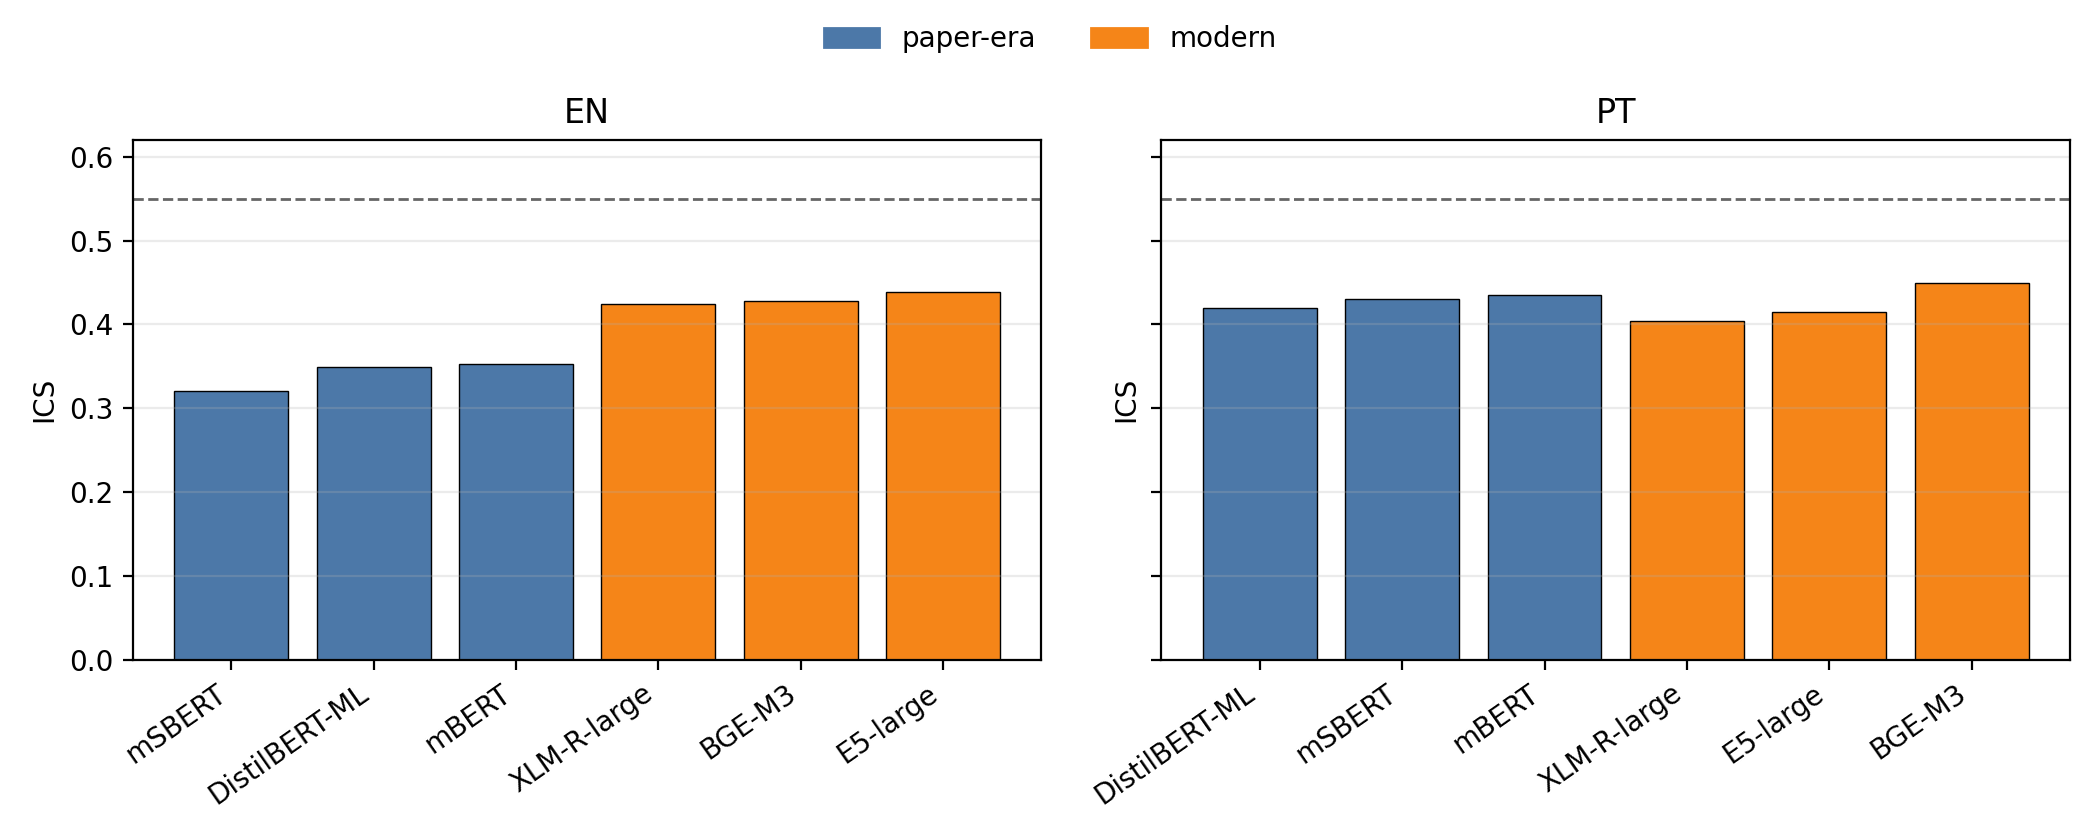
\includegraphics[width=\linewidth]{figures/ics_by_model_language.png}
\caption{Per-model ICS by language. The dashed line is the partial-capture threshold ($0.55$); no
model reaches it. The best English models (E5-large, BGE-M3) only modestly exceed the paper-era
ones, and in Portuguese the ordering is essentially flat.}
\label{fig:enc}
\end{figure}

\begin{figure}[H]
\centering
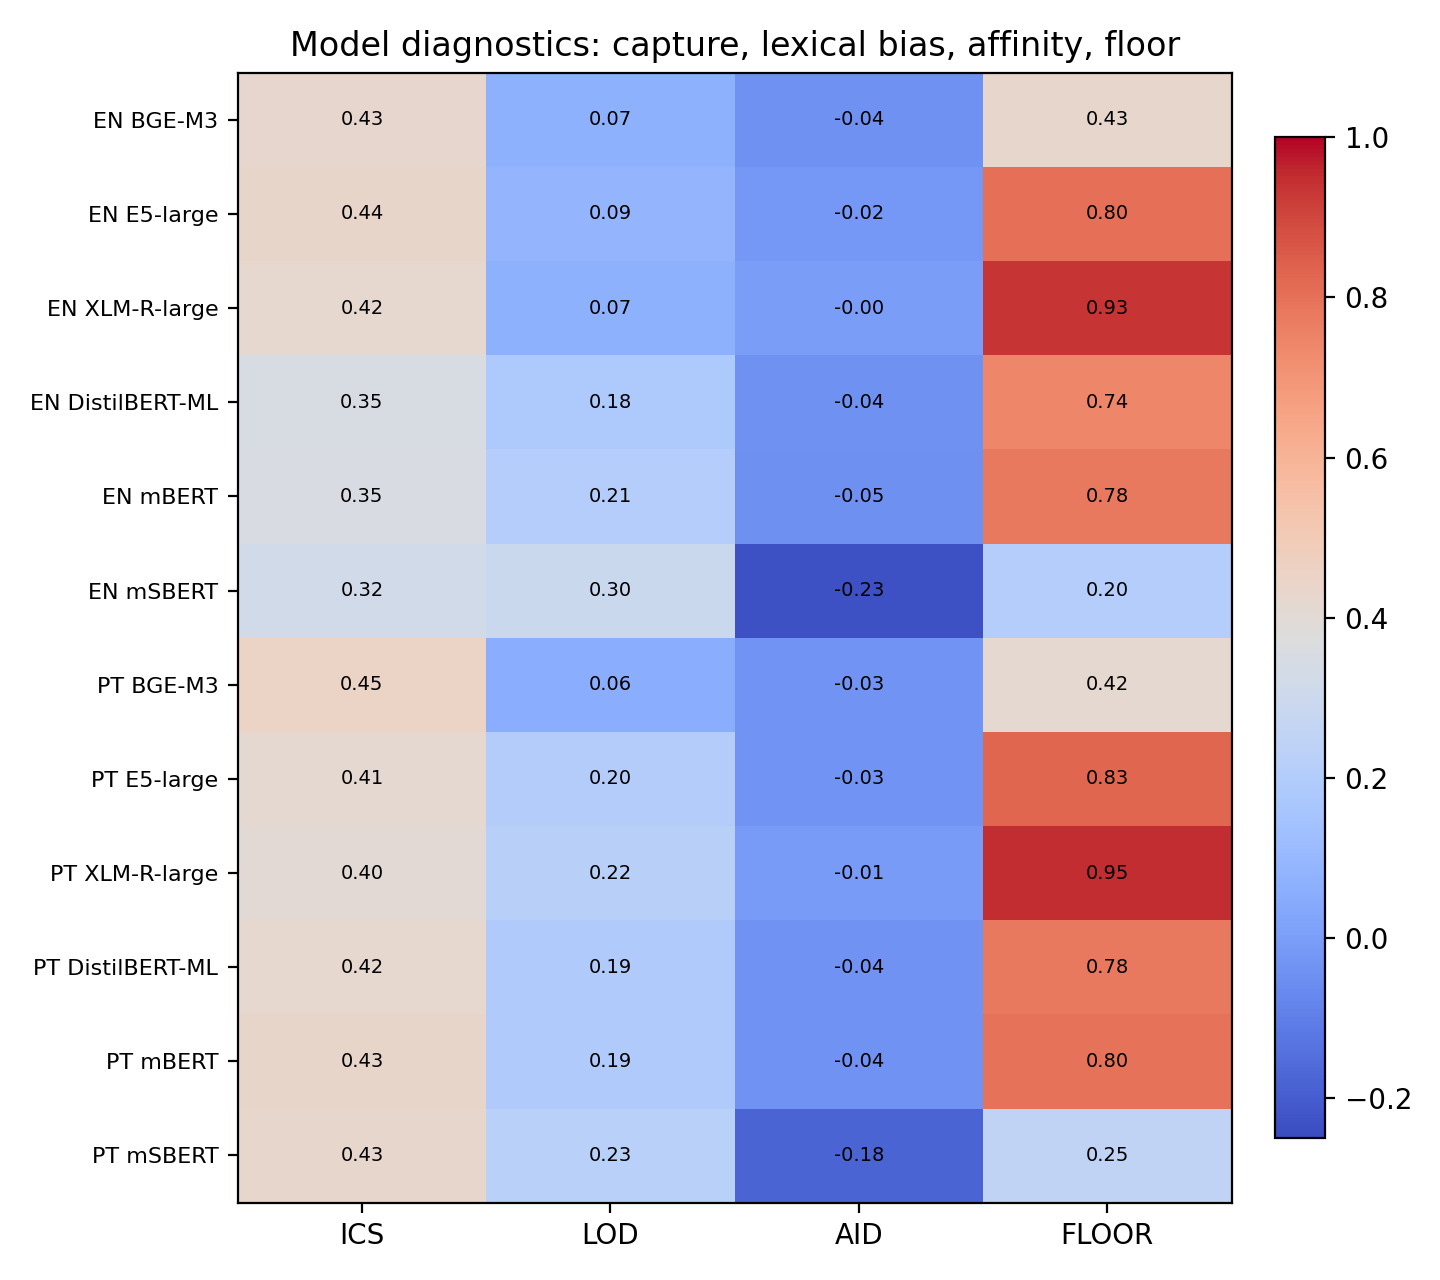
\includegraphics[width=0.82\linewidth]{figures/model_diagnostic_heatmap.png}
\caption{Diagnostic heatmap (capture, lexical bias, affinity, floor) for the encoder cohort. The
high-FLOOR rows (XLM-R-large, E5-large) show how anisotropy and lexical bias interact: a low LOD
under a near-$1$ floor is not the same as genuine idiom understanding.}
\label{fig:heat}
\end{figure}

\paragraph{Reading.} This reproduces He et al.: 2024 models do not represent idiomaticity, and the
improvement is language-dependent and small. That the English gain does not transfer to Portuguese
hints it may come from English-heavy training data rather than from genuinely learning idioms. But
these tables cannot yet separate ``the model fails on idioms'' from ``the measurement is insensitive
in general,'' which is what Experiment~4 is for.

\section{Experiment 2: Modern Sentence-Embedding Models}
\label{sec:exp2}

\paragraph{Setup and caveat.} Three 2025 and 2026 embedding models that top retrieval leaderboards:
Qwen3-Embedding-0.6B, Qwen3-Embedding-4B, and multilingual-E5-large-instruct. These produce one
pooled vector per input, so at NC level we encode the \emph{isolated phrase} (\emph{grey matter} on
its own vs \emph{brain} on its own) rather than a contextual span, a difference to keep in mind when
comparing to the encoders and LLMs.

\begin{table}[H]
\centering
\small
\begin{tabular}{lrrrr}
\toprule
Model & ISC & LOD & FLOOR & ICS \\
\midrule
Qwen3-Embedding-4B & 0.300 & 0.043 & 0.509 & \textbf{0.478} \\
mE5-large-instruct & 0.316 & 0.091 & 0.834 & 0.460 \\
Qwen3-Embedding-0.6B & 0.201 & 0.149 & 0.543 & 0.401 \\
\bottomrule
\end{tabular}
\caption{Modern embedding models on English NCIMP (isolated-phrase level). The best, Qwen3-Embedding-4B
($0.478$), slightly exceeds the strongest 2024 encoder (E5-large, $0.438$) but stays under $0.55$.}
\label{tab:emb}
\end{table}

\paragraph{Reading, with example.} Two different model families converge on the same wall:
Qwen3-Embedding-4B ($0.478$) and the decoder Qwen3-4B ($0.479$, next section) land at essentially
the same score, both with near-zero lexical bias yet both below threshold. \emph{Example of the
residual failure:} at ISC $0.30$ the gold synonym for an idiom is, on average, only $30\%$ of the way
above the random floor, a weak bridge rather than real understanding. Reducing lexical bias is not,
by itself, enough; and a healthy low floor (Qwen3-Embedding's $0.51$) is not enough either.

\section{Experiment 3: The Decoder-Only LLM Cohort}
\label{sec:exp3}

\paragraph{Setup.} Eleven models across two generations and both training stages: Qwen3 (2025) and
Qwen3.5 (2026); Gemma~3 (2025) and Gemma~4 (2026); base and instruction-tuned; 0.8B to 12B. All at
NC (contextual-span) level with the last-four-layers-plus-final-norm recipe of
Section~\ref{sec:framework}. Table~\ref{tab:llm} is generated directly from the run outputs, so the
numbers and the text cannot drift apart.

\begin{table}[H]
\centering
\small
\begin{tabular}{lllrrrr}
\toprule
Model & Gen. & Type & ISC & LOD & FLOOR & ICS \\
\midrule
Qwen3.5-0.8B-Base & 2026 & base/mlx & +0.186 & +0.101 & 0.561 & 0.425 \\
Qwen3.5-2B-it & 2026 & instruct/mlx & +0.200 & +0.060 & 0.511 & 0.444 \\
Gemma3-1B-it & 2025 & instruct/mlx & +0.207 & +0.080 & 0.667 & 0.455 \\
Qwen3.5-9B-it & 2026 & instruct/mlx & +0.217 & +0.010 & 0.540 & 0.478 \\
Qwen3-4B-Base & 2025 & base/torch & +0.188 & +0.050 & 0.825 & 0.479 \\
Qwen3.5-4B-it & 2026 & instruct/mlx & +0.222 & +0.011 & 0.523 & 0.479 \\
Gemma4-E2B-Base & 2026 & base/torch & +0.213 & +0.025 & 0.812 & 0.490 \\
Gemma3-12B-pt & 2025 & base/mlx & +0.258 & -0.006 & 0.556 & 0.498 \\
Gemma3-4B-pt & 2025 & base/mlx & +0.254 & +0.008 & 0.682 & 0.499 \\
Gemma4-12B-it & 2026 & instruct/mlx & -0.006 & +0.010 & 0.949 & 0.520 \\
Gemma4-12B-base & 2026 & base/mlx & +0.260 & -0.033 & 0.531 & 0.525 \\
\bottomrule
\end{tabular}
\caption{Decoder-only LLMs on English NCIMP (mean over contexts), sorted by ICS. Threshold $=0.55$.
The instruction-tuned Gemma~4-12B is discussed below; its high ICS is an anisotropy artefact, not
genuine capture (note its FLOOR of $0.95$).}
\label{tab:llm}
\end{table}

\paragraph{Three findings, each with an example.}
\begin{enumerate}
  \item \textbf{Nothing crosses $0.55$.} The whole cohort sits at ICS $0.42$ to $0.525$, in the same
  band as the 2024 encoders of Experiment~1.
  \item \textbf{The failure mode shifts.} Encoders fail by over-weighting literal pieces (LOD~$>0$);
  decoder LLMs push LOD to about zero. \emph{Example:} the cohort leader, base Gemma~4-12B, reaches
  LOD~$=-0.03$, the first model to put \emph{brain} closer to \emph{grey matter} than \emph{silvery
  material}, the right preference at last. Yet its ISC is only $0.26$ and its ICS $0.525$, still
  short of the bar.
  \item \textbf{Scale, generation, and alignment all approach but do not cross.} Within Qwen3.5, ICS
  saturates from about 4B onward at the 2025 Qwen3-4B value. In a like-for-like base comparison at
  12B, the newer Gemma~4 ($0.525$) modestly beats Gemma~3 ($0.498$), so a newer generation helps a
  little, but the gain is small and below threshold.
\end{enumerate}

\paragraph{The anisotropy artefact, concretely.} Instruction-tuned Gemma~4-12B reports ICS $0.520$,
which looks competitive, but its FLOOR is $0.95$: alignment tuning has collapsed its space so that
everything is about $0.95$ similar. Its genuine synonym recovery (ISC) is near $0$, and the high
composite is the metric instability of Section~\ref{sec:metrics} (dividing by $1-0.95$), not real
capture. The base version of the same model (ISC $0.26$, FLOOR $0.53$, ICS $0.525$) is the real
result. This is the second methodological finding: report FLOOR alongside ICS, always.

\section{Experiment 4: The Ordinary-Perturbation Control}
\label{sec:exp4}

\paragraph{The missing control.} Experiments 1 to 3 show models failing on idioms. But high
similarity after a small edit could be a general property of sentence embeddings, not something about
idioms. The original protocol never checks this, because its random baseline exists only for NC
targets. We add the missing comparison: run the exact same synonym-versus-random test on
non-idiomatic targets.

\paragraph{The controls, by example.} Two new groups (16 items each) join the idiomatic and
compositional compounds.
\begin{itemize}
  \item \textbf{Ordinary single words}: \emph{doctor} to \emph{physician} (synonym) vs \emph{doctor}
  to \emph{carpet} (random).
  \item \textbf{Ordinary two-word phrases}: \emph{red car} to \emph{crimson vehicle} vs \emph{red
  car} to \emph{coffee spoon}.
\end{itemize}
There is no idiomaticity here, so any competent model should easily place the synonym above the
random replacement.

\paragraph{The calibrated metric.} For a group $g$, let $\Delta_g$ be its mean synonym-minus-random
gap. The \emph{ordinary-calibrated gap} expresses the idiomatic separation as a fraction of the
ordinary one,
\[
\mathrm{OCG}_g = \frac{\Delta_g}{\Delta_{\mathrm{ordinary}}},\qquad
\Delta_{\mathrm{ordinary}}=\tfrac12(\Delta_{\text{ord.\ word}}+\Delta_{\text{ord.\ phrase}}).
\]
$\mathrm{OCG}=1$ means idioms separate as cleanly as ordinary targets; $\mathrm{OCG}$ far below $1$
means the synonym-random distinction specifically collapses for idioms.

\paragraph{Expected vs.\ actual, on one model.} For mBERT at contextual-span level, the ordinary word
\emph{doctor} separates cleanly (\emph{physician} $=0.93$ vs \emph{carpet} $=0.77$, a gap of $0.16$),
while the idiomatic group gap is $-0.01$ (the gold synonym is, if anything, slightly farther than a
random word). So mBERT's idiomatic OCG is essentially zero: the very same model that easily tells
\emph{physician} from \emph{carpet} cannot tell an idiom's gold synonym from noise.

\paragraph{Sentence level is the wrong place to look.} Before the span-level result, the control also
explains a trap. At full-sentence level, random replacements stay highly similar for \emph{every}
group, because the shared sentence frame dominates the embedding (Figure~\ref{fig:sentfloor}). So a
high sentence-level cosine is not idiomaticity evidence at all; the contextual span is where the
distinction lives.

\begin{figure}[H]
\centering
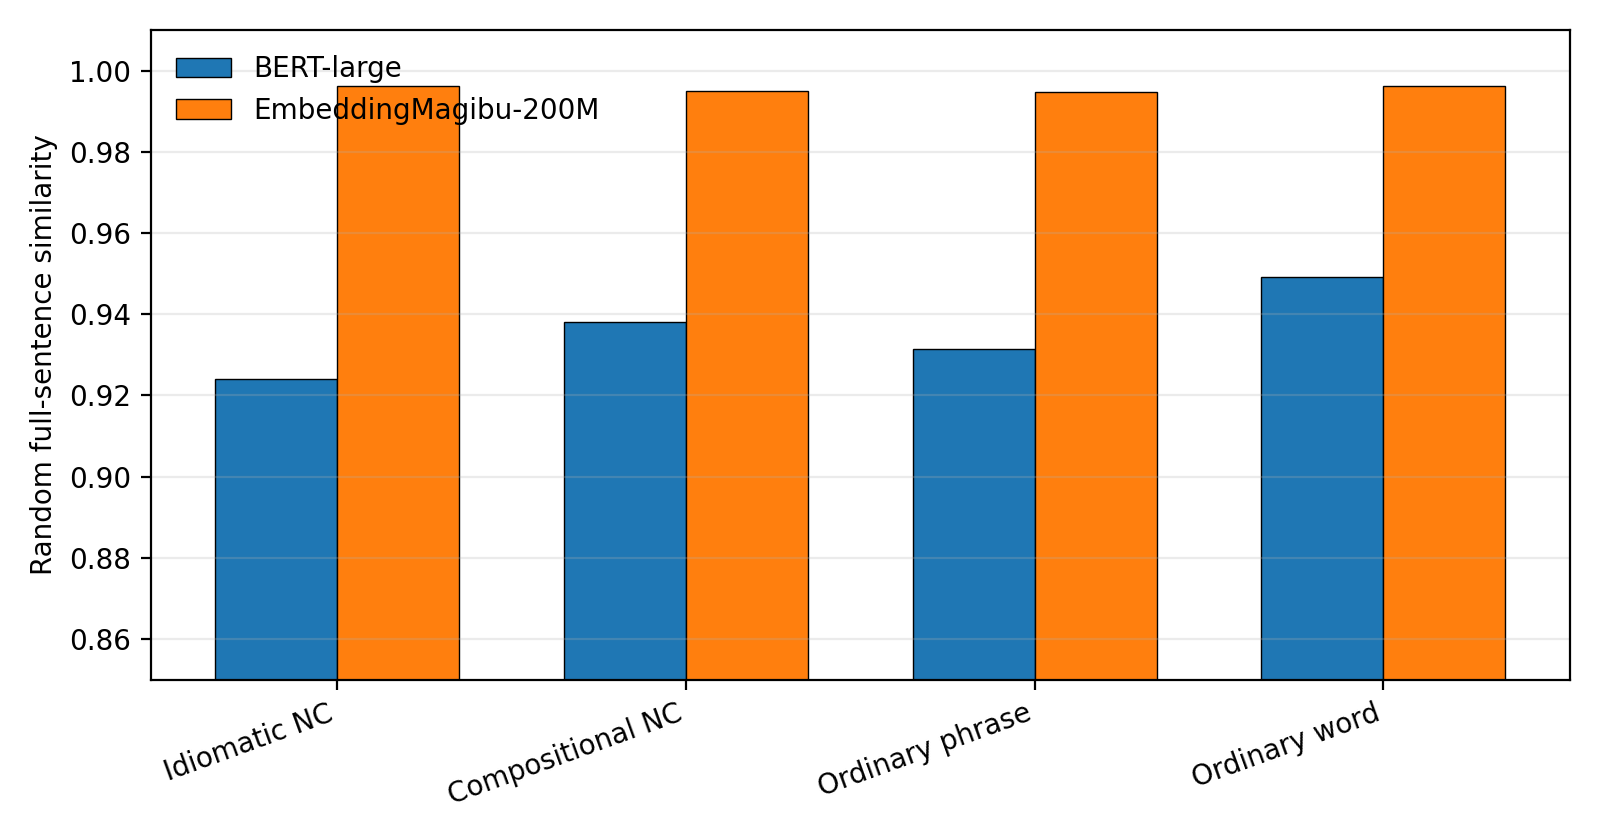
\includegraphics[width=0.82\linewidth]{figures/random_sentence_floor.png}
\caption{Random-replacement \emph{full-sentence} similarity stays high (0.90 to 0.99) for all four
groups, idiomatic and ordinary alike. The shared sentence frame, not idiomaticity, drives this; it
is why the analysis must move to the contextual span.}
\label{fig:sentfloor}
\end{figure}

\paragraph{Result across all twenty models.} Figure~\ref{fig:ocg} and Table~\ref{tab:ocg} give the
contextual-span OCG for the entire study cohort. The result is uniform: $\mathrm{OCG}_{\mathrm{idiom}}$
never reaches $1$ (best: base Gemma~4-12B at $0.68$), while the compositional calibrated gap sits at
or above $1$ for nearly every model. Compositional compounds behave like ordinary phrases; idioms do
not. The paper-era encoders are worst, at about $0$ or negative.

\begin{figure}[H]
\centering
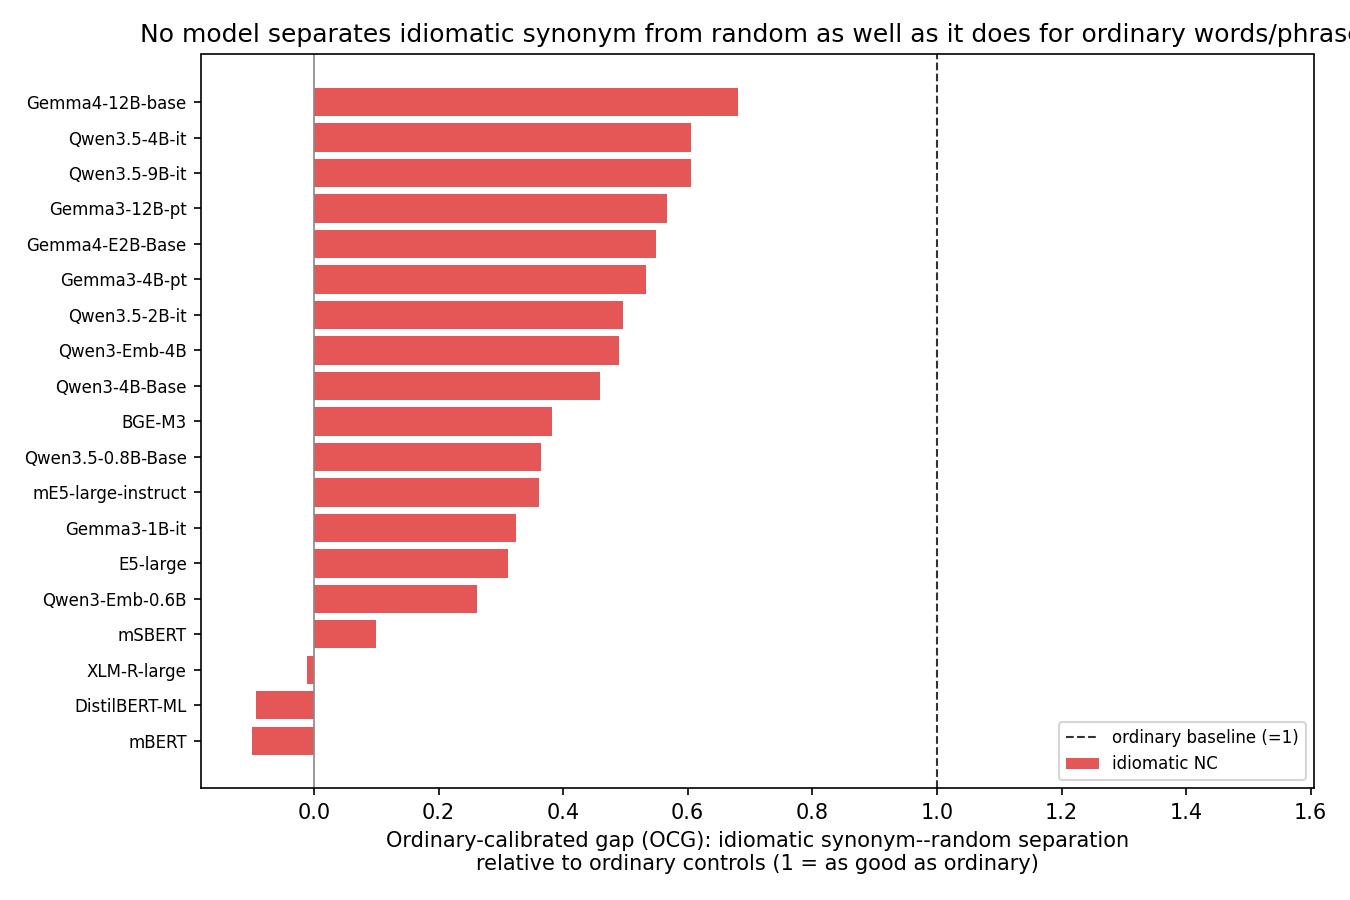
\includegraphics[width=0.92\linewidth]{figures/ocg_all_models.png}
\caption{Ordinary-calibrated idiomatic gap (OCG) for all twenty models at contextual-span level. The
dashed line at $1$ is the ordinary-control baseline. Every model falls short: the newest base LLM
(Gemma~4-12B) is closest at $0.68$, the 2024 encoders sit near or below zero. Instruction-tuned
Gemma~4-12B is omitted (its collapsed space makes the ratio unstable).}
\label{fig:ocg}
\end{figure}

\begin{table}[H]
\centering
\footnotesize
\begin{tabular}{lrrr|lrrr}
\toprule
Model & idiom gap & ord.\ gap & OCG & Model & idiom gap & ord.\ gap & OCG \\
\midrule
Gemma4-12B-base & 0.186 & 0.273 & \textbf{0.68} & Qwen3.5-0.8B-base & 0.092 & 0.252 & 0.36 \\
Qwen3.5-4B-it   & 0.147 & 0.242 & 0.61 & mE5-large-instruct & 0.042 & 0.115 & 0.36 \\
Qwen3.5-9B-it   & 0.138 & 0.229 & 0.61 & Gemma3-1B-it & 0.074 & 0.227 & 0.33 \\
Gemma3-12B-pt   & 0.155 & 0.273 & 0.57 & E5-large & 0.027 & 0.088 & 0.31 \\
Gemma4-E2B-base & 0.066 & 0.121 & 0.55 & Qwen3-Emb-0.6B & 0.070 & 0.267 & 0.26 \\
Gemma3-4B-pt    & 0.109 & 0.205 & 0.53 & mSBERT & 0.053 & 0.533 & 0.10 \\
Qwen3.5-2B-it   & 0.121 & 0.245 & 0.50 & XLM-R-large & -0.000 & 0.037 & -0.01 \\
Qwen3-Emb-4B    & 0.139 & 0.284 & 0.49 & DistilBERT-ML & -0.011 & 0.115 & -0.09 \\
Qwen3-4B-Base   & 0.054 & 0.117 & 0.46 & mBERT & -0.012 & 0.124 & -0.09 \\
BGE-M3          & 0.097 & 0.254 & 0.38 & Gemma4-12B-it$^\ast$ & 0.001 & 0.003 & 0.20 \\
\bottomrule
\end{tabular}
\caption{Ordinary-calibrated idiomatic gap for all twenty models (contextual span), sorted by OCG.
The compositional gap (not shown) is at or above the ordinary baseline for nearly all models;
$^\ast$Gemma4-12B-it has a collapsed space, so its ratio is unstable.}
\label{tab:ocg}
\end{table}

For the two-model pilot that motivated this control (BERT-large and a local embedding model), the
same picture holds at finer granularity (Figure~\ref{fig:ocgpilot}): ordinary words and phrases reach
near the baseline, idiomatic compounds reach only a fraction of it.

\begin{figure}[H]
\centering
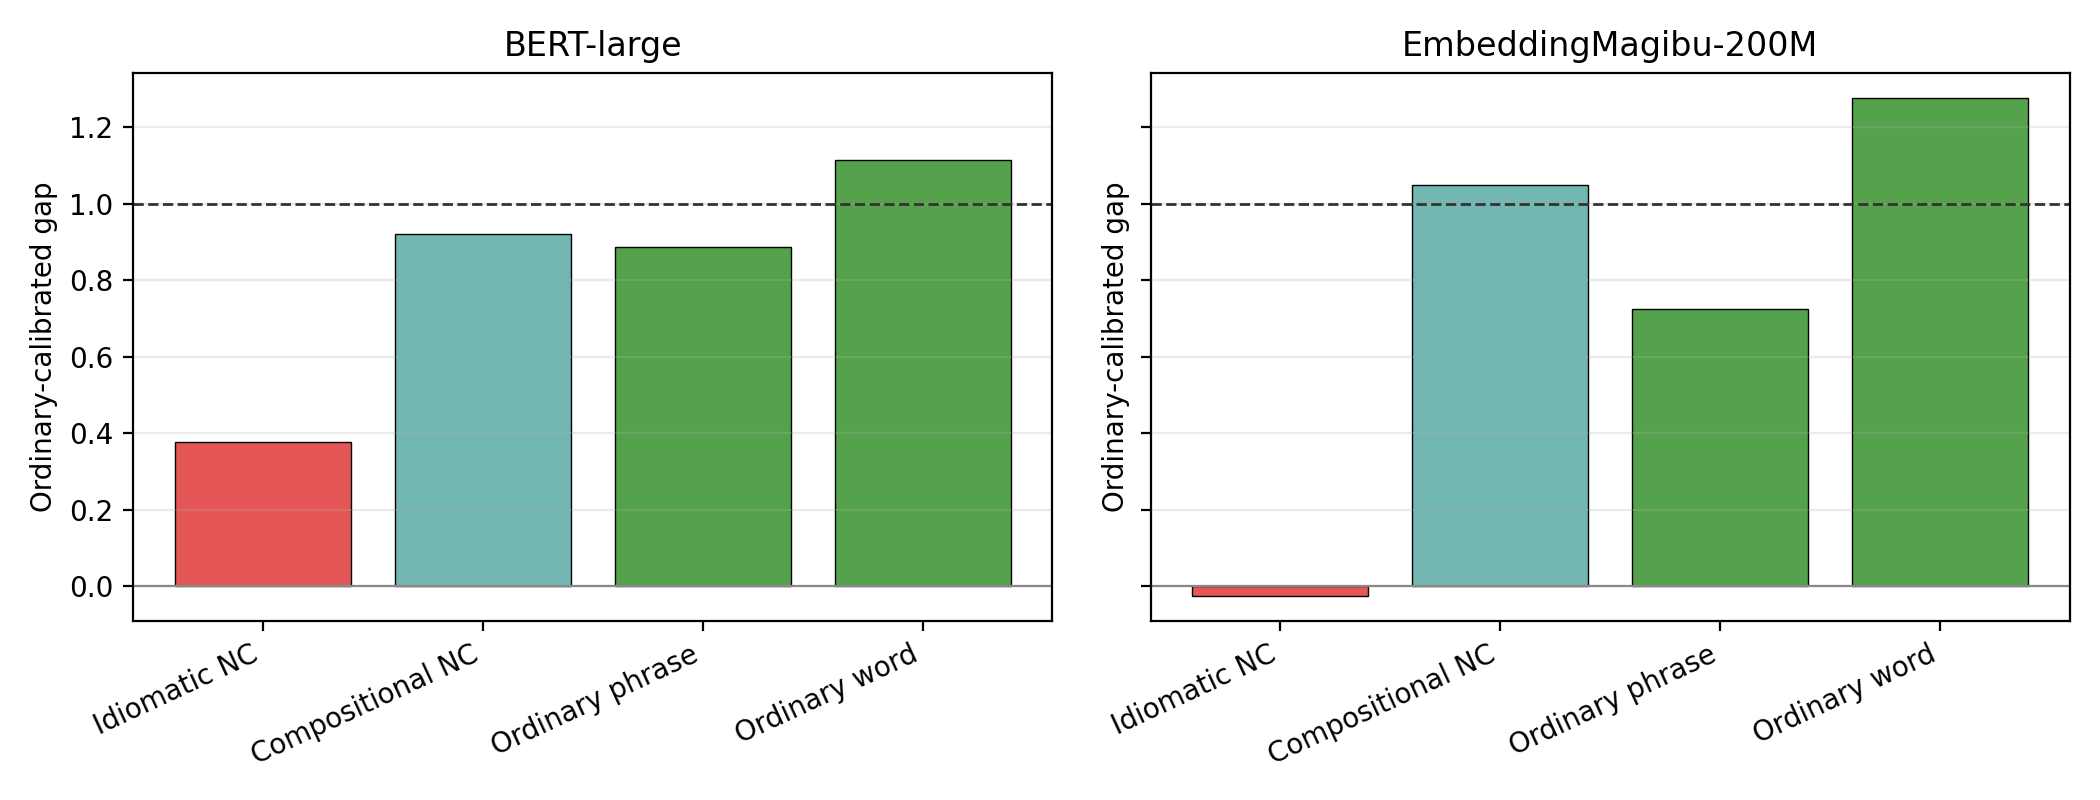
\includegraphics[width=\linewidth]{figures/ordinary_calibrated_contextual_gap.png}
\caption{The original two-model pilot. BERT-large separates ordinary controls well but idiomatic
compounds reach only about a third of the ordinary baseline; the local embedding model fails even
more strongly on idioms. This pilot motivated running the calibration on all twenty models.}
\label{fig:ocgpilot}
\end{figure}

\paragraph{Reading.} This is the cleanest single result in the study: the failure is specific to
idiomaticity (compositional and ordinary targets separate fine), and even the best modern model
recovers only two-thirds of the ordinary synonym-random separation for idioms.

\section{Putting It Together: All Twenty Models}
\label{sec:together}

Table~\ref{tab:master} collects the headline NC-level capture score for every model, across the three
modelling families, in one place. The range is narrow ($0.32$ to $0.525$) and the threshold line at
$0.55$ is never reached. Reading down the column, neither family, nor scale, nor year, nor training
stage pulls clearly ahead.

\begin{table}[H]
\centering
\footnotesize
\begin{tabular}{lll r}
\toprule
Model & Family & Year/type & ICS \\
\midrule
Gemma4-12B-base & decoder LLM & 2026 base & 0.525 \\
Gemma4-12B-it$^\ast$ & decoder LLM & 2026 instruct & 0.520 \\
Gemma3-4B-pt & decoder LLM & 2025 base & 0.499 \\
Gemma3-12B-pt & decoder LLM & 2025 base & 0.498 \\
Gemma4-E2B-base & decoder LLM & 2026 base & 0.490 \\
Qwen3.5-4B-it & decoder LLM & 2026 instruct & 0.479 \\
Qwen3-4B-Base & decoder LLM & 2025 base & 0.479 \\
Qwen3.5-9B-it & decoder LLM & 2026 instruct & 0.478 \\
Qwen3-Embedding-4B & embedding & 2025 & 0.478 \\
mE5-large-instruct & embedding & 2024 & 0.460 \\
Gemma3-1B-it & decoder LLM & 2025 instruct & 0.455 \\
Qwen3.5-2B-it & decoder LLM & 2026 instruct & 0.444 \\
E5-large & encoder/emb & 2024 & 0.438 \\
BGE-M3 & encoder/emb & 2024 & 0.428 \\
Qwen3.5-0.8B-base & decoder LLM & 2026 base & 0.425 \\
XLM-R-large & encoder & 2024 & 0.424 \\
Qwen3-Embedding-0.6B & embedding & 2025 & 0.401 \\
mBERT & encoder & 2024 & 0.353 \\
DistilBERT-ML & encoder & 2024 & 0.349 \\
mSBERT & encoder/emb & 2024 & 0.320 \\
\bottomrule
\end{tabular}
\caption{Every model in the study, English NC level, sorted by ICS. No model reaches the
partial-capture threshold of $0.55$. $^\ast$Gemma4-12B-it's score is an anisotropy artefact (FLOOR
$0.95$); its base counterpart at the top of the table is the genuine leader.}
\label{tab:master}
\end{table}

\section{Discussion}
\label{sec:discussion}

Reading the four experiments together gives a consistent, calibrated answer to ``have newer models
learned to read idioms?''
\begin{itemize}
  \item \textbf{A soft ceiling, approached from every direction.} More parameters (0.8B to 12B), a
  newer generation (2024 to 2026), a different family (encoder, embedding, decoder), and alignment
  tuning all push toward, but none past, an ICS of about $0.50$ to $0.53$. The strongest model, base
  Gemma~4-12B, is the first to get the qualitative sign right (it prefers the gold synonym) yet still
  stops at $0.525$.
  \item \textbf{The failure is specifically idiomatic.} The ordinary control rules out the deflating
  alternative that embeddings are simply insensitive to small edits: they separate \emph{doctor} to
  \emph{physician}/\emph{carpet}, and even compositional compounds, cleanly, and fail only on idioms.
  \item \textbf{The bottleneck looks structural, not a matter of capacity.} If scale were the issue,
  the 12B models would pull away; they do not. If the representation merely needed de-biasing, the
  embedding models (low lexical bias) would cross the bar; they do not. What remains is a small
  surviving synonym-random margin for idioms that newer models widen only slightly. Likely routes
  forward are therefore not bigger models but idiom-aware objectives, adapters or curricula, and
  anisotropy-corrected representations.
  \item \textbf{Two methodological lessons.} For decoder LLMs the final layer's residual stream is
  anisotropic and must be normalised, or scores are noise (Section~\ref{sec:framework}); and the
  composite ICS must be read with FLOOR, since extreme anisotropy inflates it spuriously
  (Section~\ref{sec:exp3}).
\end{itemize}

\section{Limitations}

The ordinary-control set is small (64 hand-built items) and some random replacements are
grammatically awkward; a larger, balanced version would strengthen the calibration. The composite ICS
is a heuristic for ranking, not ground truth; the per-indicator numbers (ISC, LOD, and the OCG of
Experiment~4) carry the argument. The decoder-LLM cohort is English-only at NC level; extending it to
Portuguese, where Experiment~1 already diverges from English, is the natural next step. Finally, MLX
reports the final hidden state, so its recipe (last four layers plus final norm) is close to, but not
identical with, the torch path; we keep base, full-precision weights to minimise other confounds.

\section{Conclusion}

We rebuilt the idiomaticity probe of He et al.~(2025) as a model-agnostic framework and ran it on
twenty models from 2024 encoders to 2026 LLMs, adding an MLX path for the newest architectures and a
final-norm recipe that makes decoder-LLM representations measurable. The headline is a soft ceiling:
no model captures idiomaticity, the best (base Gemma~4-12B) reaches only $0.525$ while becoming the
first to prefer the gold synonym over the literal one, and scale, generation, and alignment all
approach but do not cross the bar. An ordinary-perturbation control on all twenty models shows the
failure is specific to idioms: models separate \emph{doctor} to \emph{physician} from \emph{carpet}
cleanly but cannot do the same for an idiom's gold synonym. The original conclusion therefore stands,
now sharpened and calibrated: representing what an idiom \emph{means}, rather than what its words
\emph{say}, remains an open problem that newer and larger models have narrowed but not solved.

\appendix
\section{Reproducibility: What Was Run}
\label{sec:repro}

Every result in this paper is produced by the model-agnostic framework and saved under \texttt{runs/}
and \texttt{experiments/perturbation\_control/}. Table~\ref{tab:repro} maps each experiment to its
data, models, and outputs. All twenty models were run offline from local caches; the article tables
and figures are regenerated by a single asset-builder script, and the decoder-LLM table is written
directly from the run outputs (so it cannot drift from the text).

\begin{table}[H]
\centering
\small
\begin{tabular}{lll}
\toprule
Experiment & Models / data & Outputs \\
\midrule
1. Encoders & 6 models, EN+PT, NCIMP & \texttt{runs/en\_all}, \texttt{runs/pt\_all} \\
2. Embeddings & 3 models, EN, NCIMP & \texttt{runs/emb\_*} \\
3. Decoder LLMs & 11 models, EN, NCIMP & \texttt{runs/llm\_*}, \texttt{runs/small\_*} \\
4. Ordinary control & 20 models, 64-item control set & \texttt{experiments/perturbation\_control/all\_models} \\
\bottomrule
\end{tabular}
\caption{Experiment-to-output map. Detailed per-experiment write-ups, each with worked examples, are
in \texttt{experiments\_docs/}.}
\label{tab:repro}
\end{table}

\begin{thebibliography}{9}

\bibitem{he2025idiomaticity}
Wei He, Tiago Kramer Vieira, Marcos Garcia, Carolina Scarton, Marco Idiart, and Aline Villavicencio.
\newblock Investigating idiomaticity in word representations.
\newblock \emph{Computational Linguistics}, 51(2):505--555, 2025. doi:10.1162/coli\_a\_00546.

\bibitem{devlin2019bert}
Jacob Devlin, Ming-Wei Chang, Kenton Lee, and Kristina Toutanova.
\newblock BERT: Pre-training of deep bidirectional transformers for language understanding.
\newblock In \emph{Proceedings of NAACL-HLT}, pages 4171--4186, 2019.

\bibitem{conneau2020xlmr}
Alexis Conneau et al.
\newblock Unsupervised cross-lingual representation learning at scale.
\newblock In \emph{Proceedings of ACL}, pages 8440--8451, 2020.

\bibitem{reimers2019sbert}
Nils Reimers and Iryna Gurevych.
\newblock Sentence-BERT: Sentence embeddings using Siamese BERT-networks.
\newblock In \emph{Proceedings of EMNLP-IJCNLP}, pages 3982--3992, 2019.

\bibitem{qwen3}
Qwen Team, Alibaba Group.
\newblock Qwen3 technical report.
\newblock arXiv preprint, 2025.

\bibitem{gemma3}
Gemma Team, Google DeepMind.
\newblock Gemma 3 technical report.
\newblock arXiv preprint, 2025.

\end{thebibliography}

\end{document}
